\section{Types of Motion}
\label{sec:motion}

\noindent The first parameter investigated was the friction perpendicular to the leaf. When this parameter was varied five different types of motion were observed. For each of these the remaining four parameters were constant with $f=100, l=1, \rho = 0.1, g = 9.81$. The initial conditions also remained constant with $u=v=\omega=x=y=0$ and $\theta=1$.
\noindent The first motion is displayed in Figure \ref{fig:Motion1}, for this motion the friction coefficient perpendicular to the leaf was set at 4.84. 

\begin{figure}[H]
\centering
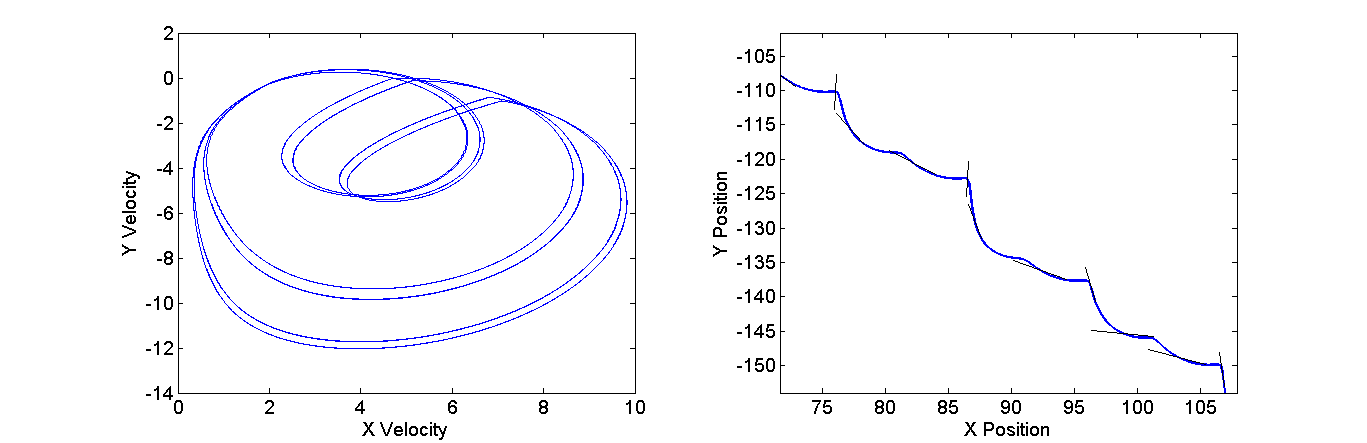
\includegraphics[width=0.7\textwidth]{Motion_Graphs/Motion1.png}
\caption{\label{fig:Motion1}(Left)Plot showing the velocity in the x and y direction after transients have decayed. (Right) Plot showing the position of the leaf in the x and y direction after transients have decayed. The solid line shows the trajectory of the leaf while the short lines indicate the orientation of the leaf.%%say how often each of these is plotted? Use better term than "short lines"
}
\end{figure}

\noindent As Figure \ref{fig:Motion1} shows the leaf falls regularly to the right while rotating. The direction of the fall and rotation depend on the initial conditions, if the initial values remain the same, except $\theta=-1$ then the leaf will fall to the left. The velocity of the leaf settles to a limit cycle with a period of eight once the transients have decayed. 
% Could we analyse the limit cycle for stability?

\noindent When the value of the friction coefficient perpendicular to the leaf is increased to 4.9 the motion of the leaf does not appear to show any significant change. However the the limit cycle becomes much denser, this is shown in Figure \ref{fig:Motion2}. %Is this still a limit cycle they call it a strange attractor in the report.

\begin{figure}[H]
\centering
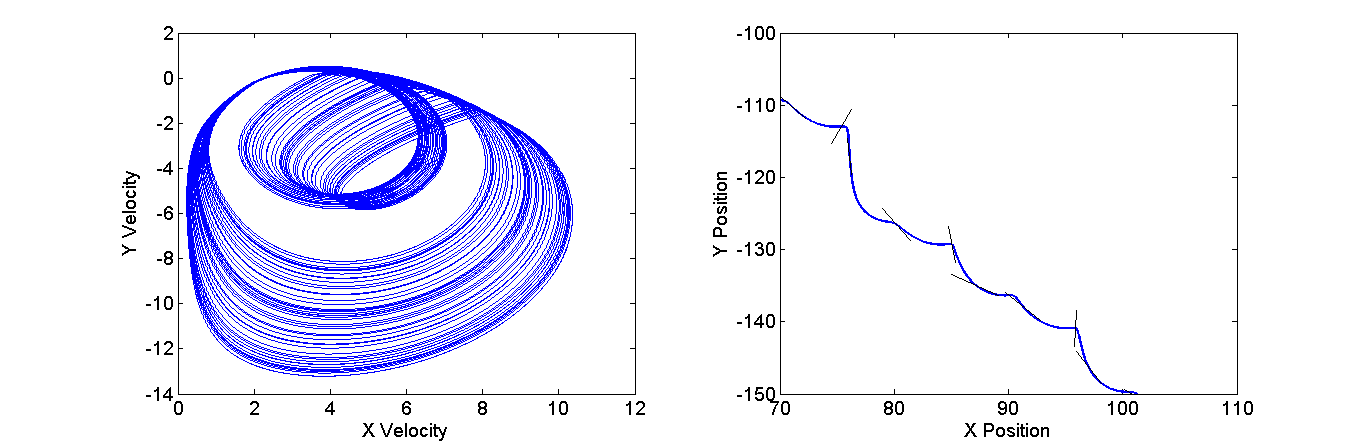
\includegraphics[width=0.7\textwidth]{Motion_Graphs/Motion2.png}
\caption{\label{fig:Motion2}(Left)Plot showing the velocity in the x and y direction after transients have decayed. (Right) Plot showing the position of the leaf in the x and y direction after transients have decayed. The solid line shows the trajectory of the leaf while the short lines indicate the orientation of the leaf.
}
\end{figure}

When the friction coefficient perpendicular to the leaf is increased further to 9.75 the motion of the falling leaf changes. The leaf no longer shows a regular falling pattern, instead the leaf appears to fall with no particular pattern. The leaf will fall regularly in one direction for a short period before falling with a swaying motion. Similarly the plot of the velocity changes, showing a strange attractor with symmetry about y-axis, as shown in Figure \ref{fig:Motion3}. 

\begin{figure}[H]
\centering
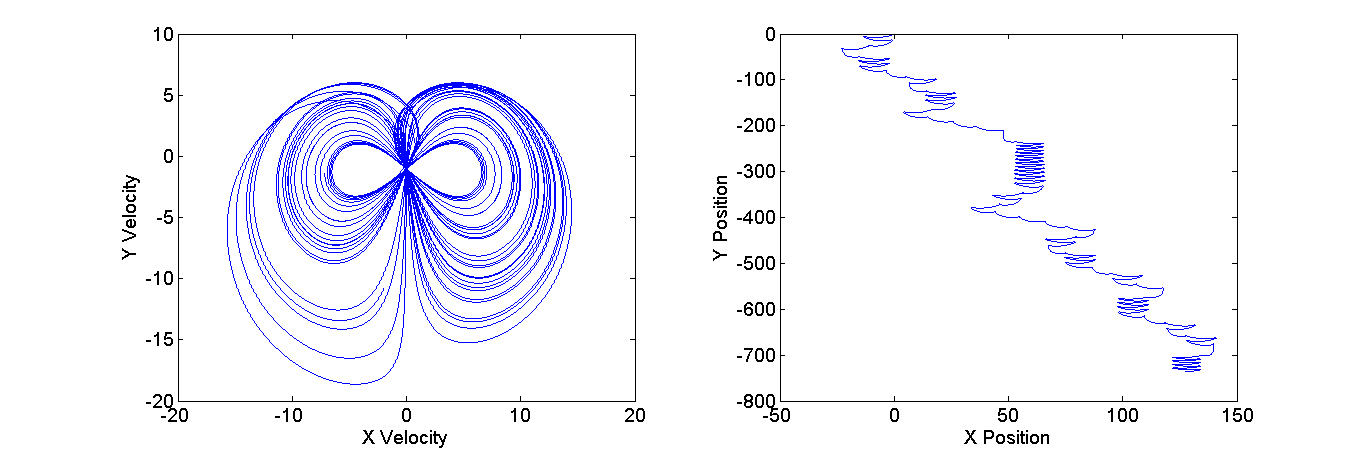
\includegraphics[width=0.7\textwidth]{Motion_Graphs/Motion3.png}
\caption{\label{fig:Motion3}(Left)Plot showing the velocity in the x and y direction after transients have decayed. (Right) Plot showing the position of the leaf in the x and y direction after transients have decayed.
}
\end{figure}

As the friction coefficient perpendicular to the leaf is increased further the motion of the leaf becomes regular again. When the coefficient is increased to 12 the leaf sways from side to side as it falls. The amplitude of the sway decreases until it settles. The leaf then falls vertically swaying with a constant amplitude. The plot of the velocity shows a similar shape to the previous motion with the symmetry about the y-axis. This is shown in Figure \ref{fig:Motion4}.

\begin{figure}[H]
\centering
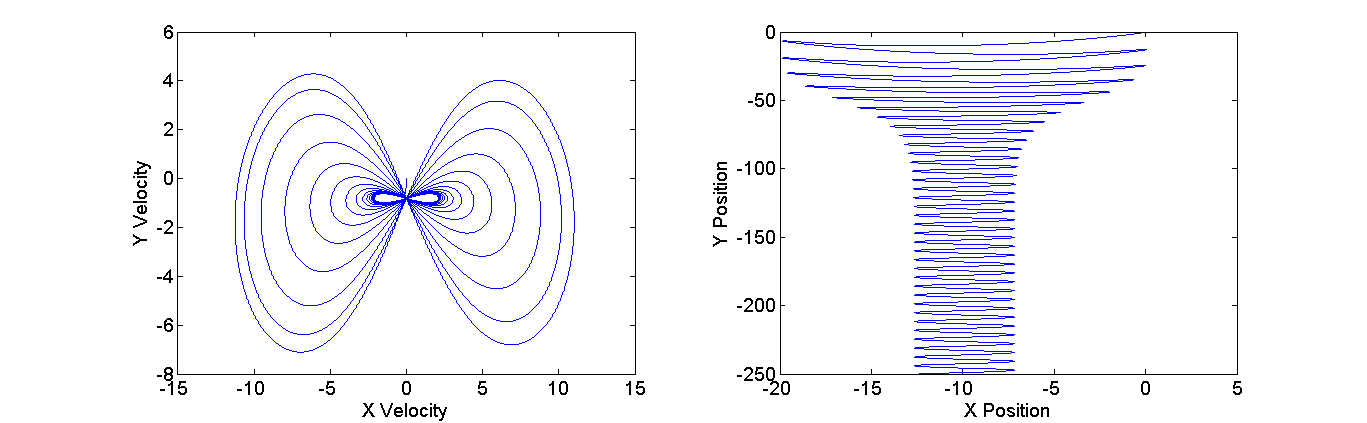
\includegraphics[width=0.7\textwidth]{Motion_Graphs/Motion4.png}
\caption{\label{fig:Motion4}(Left)Plot showing the velocity in the x and y direction after transients have decayed. (Right) Plot showing the position of the leaf in the x and y direction.
}
\end{figure}

For a further increase in the coefficient the leaf no longer sways. Instead it falls regularly to the left before it falls straight down with no change in angle and no swaying. The velocity starts at zero from the initial conditions, the magnitude of the velocity then increases before it decreases as the leaf falls with no movement in the x direction. This motion is shown in Figures \ref{fig:Motion5} and \ref{fig:Motion6}. The leaf now appears to fall with a constant angle and velocity. 

\begin{figure}[H]
\centering
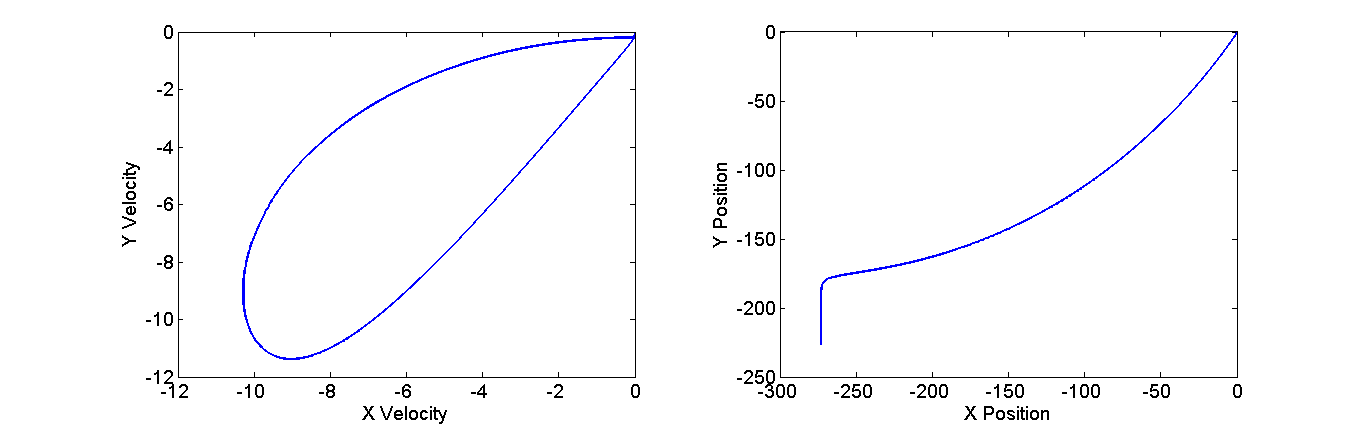
\includegraphics[width=0.7\textwidth]{Motion_Graphs/Motion5.png}
\caption{\label{fig:Motion5}(Left)Plot showing the velocity in the x and y direction after transients have decayed. (Right) Plot showing the position of the leaf in the x and y direction.
}
\end{figure}

\begin{figure}[H]
\centering
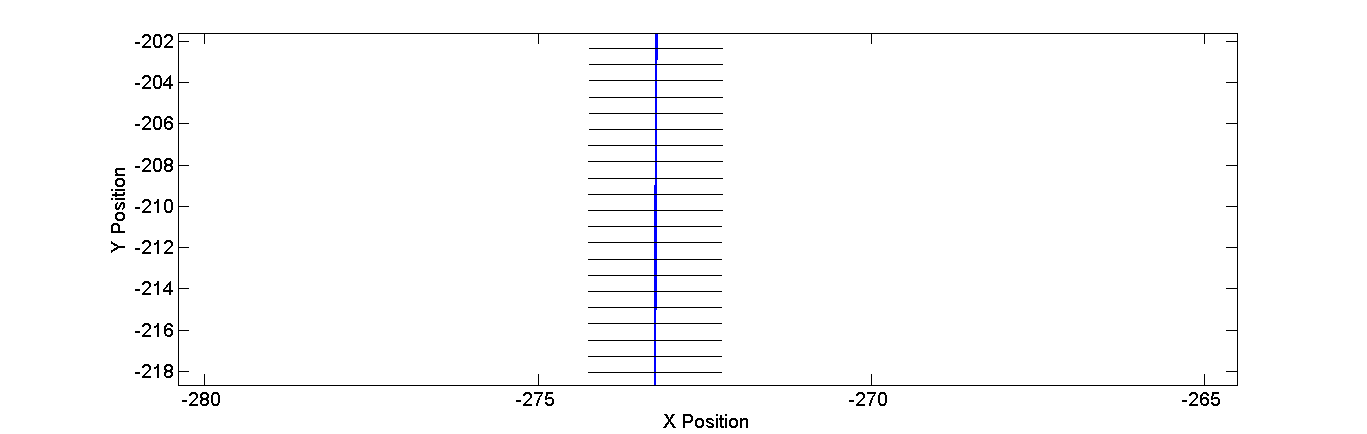
\includegraphics[width=0.7\textwidth]{Motion_Graphs/Motion6.png}
\caption{\label{fig:Motion6}Plot showing the position of the leaf in the x and y direction during the vertical fall. The solid line shows the trajectory of the leaf while the short lines show the orientation of the leaf.
}
\end{figure}



